\chapter{Performance Engineering and Optimisation}
\label{ch:optimization}

The renderer validated in \Cref{ch:validation} is fast by design; this chapter documents the
engineering behind that speed. Two kinds of claim appear, and they are justified differently.
Every kept \emph{optimisation} is measured by switching it on and off inside this renderer;
the reference plays no part in those measurements. The \emph{architecture} itself
(\Cref{ch:architecture}) is not ablated internally: its alternative is the reference's entire
segment-marching algorithm, so it is justified by complexity arguments
(\Cref{sec:complexity}) and by the end-to-end comparison of \Cref{ch:results}. The closest
internal ablations of the architecture are the cap-free collection variant
(\Cref{sec:autopsies}) and the shell-geometry A/B (\Cref{sec:icosphere}). The chapter closes with the failed attempts (\Cref{sec:autopsies}), which indicate where
effort on this class of renderer is wasted.

\section{The starting gap and the bottleneck}
\label{sec:bottleneck}

Nsight Compute (NVIDIA's kernel-level profiler) locates the bottleneck firmly in
\emph{memory latency}: the kernel is latency-bound on scattered global loads of the per-primitive
\texttt{Primitive} struct. Occupancy is $21$--$31\%$ (asset-dependent; \Cref{sec:gpu-ray-tracing} defines warps,
lanes, and occupancy), itself capped by the code-intrinsic register
pressure of the erf and phase-function chains. The primitive data is already
$\mathrm{L1}\approx\SI{82}{\percent}$, $\mathrm{L2}\approx\SI{99}{\percent}$
resident (Nsight Compute sector hit rates), so reducing its \emph{footprint} cannot help much---the cost is in the latency of
gathering scattered primitives, not in bandwidth. The same diagnosis
shaped the architecture (\Cref{sec:gpu-impl}): the per-bounce arithmetic is cheap but the per-ray state
is large and persistent, so the algorithm is \emph{megakernel-shaped}. Several of the null results
in \Cref{sec:autopsies} follow from this diagnosis alone.

Profiling the production binary quantifies this (Nsight Compute, base-clocked, one capture per asset; the kernels are deterministic, so the
coarse utilisation picture is reproducible, but the percentages below are single captures; no repeats were taken). Occupancy is low on every asset. On the showcase cloud the render megakernel reaches
$31.2\%$ occupancy at $45.9\%$ SM and $16.5\%$ DRAM throughput, and ray divergence leaves only
$5.4$--$6.9$ of $32$ lanes active per warp.\footnote{The \num{25600}-primitive bunny is the
extreme: $20.9\%$ occupancy, a scheduler that finds no eligible warp in $70\%$ of cycles, and
DRAM at $1.8\%$.} None of the four production assets approaches either roof of the arithmetic
roofline (\Cref{fig:roofline}). All sit at $0.2$--$3\%$ of the RTX~3090's FP32 compute peak and from
$0.6\%$ (tornado) to $16.5\%$ (cloud) of its bandwidth. The regime is unambiguously \emph{latency-bound}
and divergence-dominated---not compute- or bandwidth-bound. Of the two fully profiled, the bunny is the
harder case because its dense, finely-divided shell maximises traversal divergence while touching almost
no DRAM (the sparse tornado sits lower still on the roofline). This divergence is the case OptiX Shader Execution Reordering~\cite{NvidiaSER2022} is built for: regrouping
threads between traversal and shading to restore warp coherence. It is an Ada-generation feature,
unavailable on the Ampere RTX~3090 the development and validation use here. Its effect is therefore measured separately,
directly on an Ada GPU, in \Cref{sec:ser}.

\begin{figure}[htp]
  \centering
  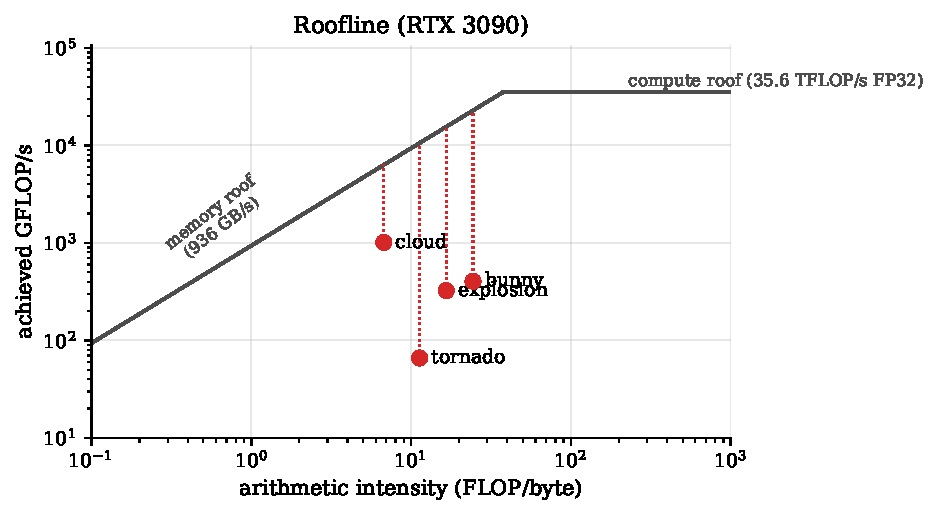
\includegraphics[width=0.7\linewidth]{figures/roofline.pdf}
  \caption{Arithmetic roofline (RTX~3090: ${\approx}35.6$~TFLOP/s FP32, ${\approx}936$~GB/s) for the
  render megakernel across the four production assets. All sit far below both roofs---achieving
  ${\approx}0.07$--$1.0$~TFLOP/s at arithmetic intensities of ${\approx}7$--$24$~FLOP/B---a
  non-saturation argument for the latency-bound diagnosis. (A roofline bounds a kernel's
attainable arithmetic throughput by the lower of two ceilings: peak compute, and
arithmetic intensity---FLOPs per byte of memory traffic---times peak bandwidth. Points far
below both indicate a limit that is neither: here, latency.) FLOPs are estimated the standard Nsight way: per-pipe instruction counters (the GPU's
arithmetic execution units) $\times$ average active lanes. The transcendental \texttt{erf}
runs on a pipe the count excludes, so the figure understates true arithmetic. Cloud is the scattering showcase ($900\times600$, \num{16}~spp);
  tornado, explosion, and bunny use the asset-validation recipe ($256\times256$, \num{4}~spp).}
  \label{fig:roofline}
\end{figure}

\section{A taxonomy of optimisations}
\label{sec:four-modes}

Not every choice warrants its own controlled measurement. An on/off ablation is worth
running only when its outcome is not a foregone conclusion; otherwise the defensible justification is a
complexity argument or a citation to standard practice. Each optimisation in this chapter is therefore
placed in one of three modes (\Cref{tab:four-modes}):

\begin{table}[htp]
  \centering
  \resizebox{\linewidth}{!}{%
  \begin{tabular}{@{}lll@{}}
    \toprule
    Mode & When it applies & Examples \\
    \midrule
    \textbf{(M) Measured} & genuine choice, non-obvious outcome & RIS, RR depth, shell geometry, autopsies \\
    \textbf{(C) Complexity-argued} & asymptotically better; argue the bound & argmin sampler, $O(1)$ active set \\
    \textbf{(S) Standard practice} & textbook; cite, do not measure & multi-stream, FMA, coalescing, fast-math \\
    \bottomrule
  \end{tabular}%
  }
  \caption{The three justification modes: optimisations are measured when the outcome is
  uncertain, argued by complexity when it is bounded, and cited when they are standard practice.}
  \label{tab:four-modes}
\end{table}

\section{Measured wins}
\label{sec:wins}

The kept speedups are summarised in \Cref{tab:wins}. All are measured \emph{within this renderer}:
each is a controlled on/off ablation against its own validated baseline, not against the
reference. Five of the six rows are development-time interleaved A/Bs of the two builds on
the scattering cloud (steady-state, correctness re-verified after
each change). The RR-depth row is the controlled \num{16}-seed campaign sweep of
\Cref{fig:rr-depth}. The caption of \Cref{tab:wins} states the provenance per row. Each row
is described here under its table name.
\begin{description}
  \item[Shadow-ray transmittance.] Profiling showed ${\sim}85\,\%$ of frame time in the shadow-ray
  optical-depth integration, which mirrored the primary-ray path: build an event list, sort, and
  march segment by segment---$O(A^2)$ erf evaluations for $A$ overlapping primitives. A shadow ray
  needs only the \emph{total} optical depth, and optical depth is additive across primitives, so each
  primitive can be integrated once over its full chord: $O(A)$. The equality is exact,
  \[
    \tau_{\mathrm{tot}} \;=\; \int_{0}^{L}\sum_i \sigma_i(t)\,\mathrm{d}t
    \;=\; \sum_i \int_{[0,L]\,\cap\,[a_i,b_i]} \sigma_i(t)\,\mathrm{d}t,
  \]
  where $[0,L]$ is the shadow segment and $[a_i,b_i]$ the interval in which the ray runs inside
  primitive $i$: each primitive contributes only where the two overlap, regardless of how the
  chords interleave. The rewrite changes the cost, not the value being computed. Rewriting the evaluation this way is
  a $\sim$\num{12}--\num{15}$\times$ speedup of the shadow kernel itself (images identical to the
  pre-change baseline up to floating-point summation order). The kernel was ${\sim}85\,\%$ of
  frame time, so the frame as a whole shortens \num{4}--\num{5}$\times$: the untouched
  \num{15}\,\% now dominates (Amdahl's law).
  \item[Skip per-bounce containment scan.] The sampler scanned all $N$ primitives at \emph{every}
  bounce to find the set containing the ray origin. After a scatter, the next bounce starts exactly
  at the scatter point, whose containing set the sampler already holds---so the scan is needed only
  at bounce~$0$ and later bounces inherit the set (the remaining bounce-$0$ scan is
measured directly in \Cref{sec:results-scaling}). ${\sim}16\,\%$ frame time; unbiased (furnace-pass,
  converged means unchanged) though not bit-identical. The inherited chord membership and a fresh
  point-containment test can disagree on boundary-grazing primitives at float precision. That
  alters the sample stream but not its distribution---the only kept change in that category.
  \item[Dedup bounce-0 scan.] At bounce $0$ the analytic-direct term re-ran the \emph{same} full-scene
  containment scan the sampler had just performed for the same origin; handing the sampler's set to
  it removes the duplicate. ${\sim}8\,\%$ frame time, bit-level image agreement.
  \item[Any-hit transmittance fusion.] Shadow rays originally filled the per-ray hit buffer during
  traversal and integrated afterwards; a transmittance-mode any-hit instead accumulates each entered
  primitive's optical depth \emph{during} the single traversal, so the buffer is never touched.
  ${\sim}3\,\%$, exact (additivity makes the accumulation order-independent).
  \item[Fast erf.] An opt-in polynomial approximation replacing the \texttt{erf} intrinsic in the hot
  path; ${\sim}1\,\%$ standalone and numerically free at render precision (kept opt-in,
  default exact).
  \item[Russian-roulette start depth.] Russian roulette is the standard unbiased way to end paths: beyond a chosen bounce depth,
  each path survives only with some probability, and survivors are reweighted to compensate.
  The start depth is a free knob. Raising it keeps more deep bounces, which lowers variance
  but costs time. This renderer raises it from the inherited surface-rendering default of $5$
  to $12$; the controlled sweep (\Cref{fig:rr-depth}) shows \emph{why} this is the right setting,
  and it also revises the magnitude of the win.\footnote{Raw basis; the recorded clip basis reproduces the same shape. Protocol on
\Cref{fig:rr-depth}.} Variance falls and frame time rises monotonically with depth.
  Their product is a \emph{flat basin}: depths $8$--$12$ are statistically tied, and every
  depth outside the basin is measurably worse (\Cref{fig:rr-depth}). The shipped default $12$
  sits at the basin's deep edge, the lower-per-sample-variance end at equal efficiency. The
  controlled sweep also revises the informal development-time estimate of the
  depth-$5\!\to\!12$ gain from ${\sim}11\,\%$ down to $+4.1\,\%$.
\end{description}
With these wins in place, and the MIS direct-lighting estimator of \Cref{sec:direct-lighting}
(improved further by the opt-in product-RIS of \Cref{sec:ris}), the renderer reaches the
reference's noise level in less time on the environment-lit showcase. That is the equal-quality
result quantified in \Cref{ch:results}.

\begin{table}[htp]
  \centering
  \resizebox{\linewidth}{!}{%
  \begin{tabular}{@{}ll@{}}
    \toprule
    Optimisation & Effect \\
    \midrule
    Shadow-ray transmittance         & $\sim$\,12--15$\times$ (shadow-kernel time) \\
    Skip per-bounce containment scan & $\sim$\,16\% frame time \\
    Russian-roulette depth $5\to12$  & $+4.1$\,\% efficiency, $k\cdot t$ (\Cref{fig:rr-depth}) \\
    Dedup bounce-0 scan              & $\sim$\,8\% frame time \\
    Any-hit transmittance fusion     & $\sim$\,3\% frame time \\
    Fast \texttt{erf} in the hot path & $\sim$\,1\% frame time (opt-in) \\
    \bottomrule
  \end{tabular}%
  }
  \caption{Measured optimisations kept in the renderer. Each is a controlled on/off ablation
  on the scattering cloud. Provenance: the RR-depth row is the campaign's $16$-seed efficiency sweep
  of \Cref{fig:rr-depth} (independently re-measured, revising an earlier development-time
  ${\sim}11\,\%$ estimate); the remaining rows are development-time A/B measurements from the repository's
  development log---a later attempt to re-measure them from the merge history was inconclusive at
  production scale, and the fast-erf figure sits at the timing-jitter floor.}
  \label{tab:wins}
\end{table}

\begin{figure}[htp]
  \centering
  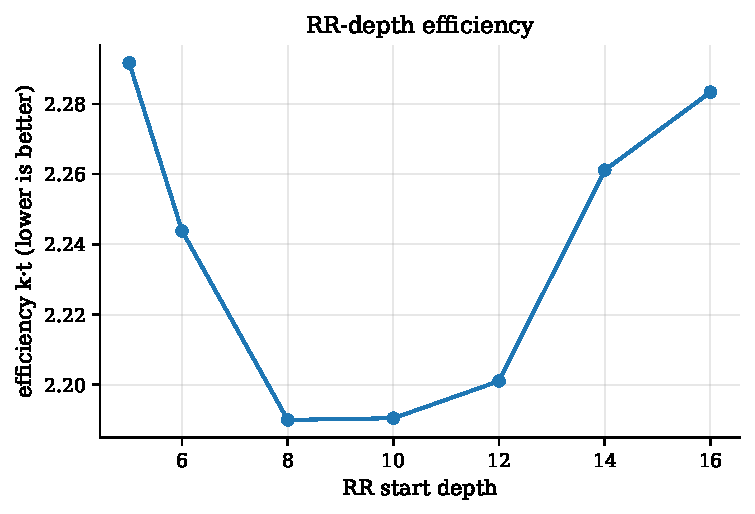
\includegraphics[width=0.8\linewidth]{figures/rr_depth.pdf}
  \caption{Russian-roulette efficiency on the scattering cloud: $k\cdot t$ (inter-seed noise constant
  $\times$ relative frame time, lower is better) against the RR start depth; the noise constant $k$ is from
  $16$ seeds per depth at \num{64} spp and the relative frame time is the median of $5$ interleaved rounds,
  under the meadow-lit showcase, sampled at depths $\{5, 6, 8, 10, 12, 14, 16\}$. The product forms a flat basin over depths $8$--$12$ (spread ${\approx}0.5\,\%$, below the
  $1$--$2\,\%$ timing spread of the rounds, so the interior ordering is not statistically resolvable),
  with both edges measured and worse ($5$: $+4.6\,\%$, $14$: $+3.2\,\%$, $16$: $+4.3\,\%$). The shipped
  default $12$ sits at the basin's deep edge, the lower-per-sample-variance end (${\sim}10\,\%$
  lower per-sample variance than depth $8$ at the same $k\cdot t$).}
  \label{fig:rr-depth}
\end{figure}

\section{The algorithmic highlight: volumetric product-RIS}
\label{sec:ris}

The chapter's one algorithmic win is in direct lighting; it is measured below.
\textbf{The technique.} The baseline next-event estimator spends
one shadow ray per scattering vertex, on an environment direction drawn by luminance. Resampled
importance sampling (RIS)~\cite{Talbot2005} improves the \emph{direction} before paying for the ray.
It draws $K$ candidate directions from the environment and scores each with a cheap target:
phase-function value $\times$ environment luminance, the integrand's inexpensive factors. It keeps
one candidate with probability proportional to its score, via a weighted
reservoir~\cite{Bitterli2020}, and traces the
single expensive shadow ray only for the survivor. $K$ cheap evaluations buy one
better-aimed ray. The reservoir performs single-frame candidate selection only; no
spatiotemporal reuse (ReSTIR) is involved.

\textbf{Goal:} measure whether product-RIS beats plain MIS at equal quality, and choose $K$.

\textbf{Setup:} the environment-lit showcase. The RIS arm and the plain-MIS baseline are
rendered at \num{64}\,spp over \num{16} independent seeds for each candidate count
$K\in\{1,2,4,6,8,12\}$, giving each arm's noise constant $k$. Frame times come from interleaved timed
rounds at the fixed operating point. The equal-quality speedup is the $k\cdot t$ ratio, with a
\num{95}\,\% bootstrap confidence interval over the seeds (both per the conventions of
\Cref{sec:setup}).

\textbf{Result:} product-RIS wins at equal quality: a statistically tied plateau of
$\mathbf{{\approx}1.48\times}$ across $K=4$--$6$, with a real decline beyond
it.\footnote{$K{=}4$: $1.481\times$, CI $[1.47, 1.49]$; the shipped default $K{=}6$:
$1.475\times$, $[1.47, 1.48]$.} Candidate cost rises
monotonically with $K$ while variance falls, and their product peaks where the proposal quality
saturates. The win decomposes into both halves: one shadow ray instead of two ($-21\,\%$ frame time),
\emph{plus} lower variance from the resampling ($-14\,\%$ noise constant). The $K{=}1$ anchor (plain environment-IS---environment-importance-sampled---NEE) already wins $1.19\times$ on time alone, \emph{despite} higher variance, which
isolates the resampling's contribution.

\textbf{Scene dependence.} The technique's value depends on the environment. A three-point
\emph{peakiness} sweep puts numbers on this dependence (\Cref{fig:ris-ksweep}); peakiness is
each environment's peak radiance relative to its mean. On a flat (constant) environment, where the
candidates are interchangeable, it is a net loss at every $K$ (best case $1.8\times$ \emph{worse},
degrading to ${\sim}12\times$ at $K{=}1$). On a mid-peak studio environment (peak ${\sim}540\times$
the mean) it already wins
$1.45\times$; on the high-peak showcase (${\sim}1.5{\times}10^{5}\times$ the mean), $1.48\times$. The win thus rises
with environment peakiness and \emph{saturates} between the studio and showcase points despite a
${\sim}300\times$ difference in peak. It is therefore
shipped behind a runtime flag (default off, plain MIS; $K=6$ the conservative default), not as an
unconditional change.
The result was validated unbiased against the Mitsuba-analog ground truth on a constant environment
(furnace-clean) \emph{and} on the environment-lit showcase (converged means within the Monte Carlo
noise floor).

\begin{figure}[htp]
  \centering
  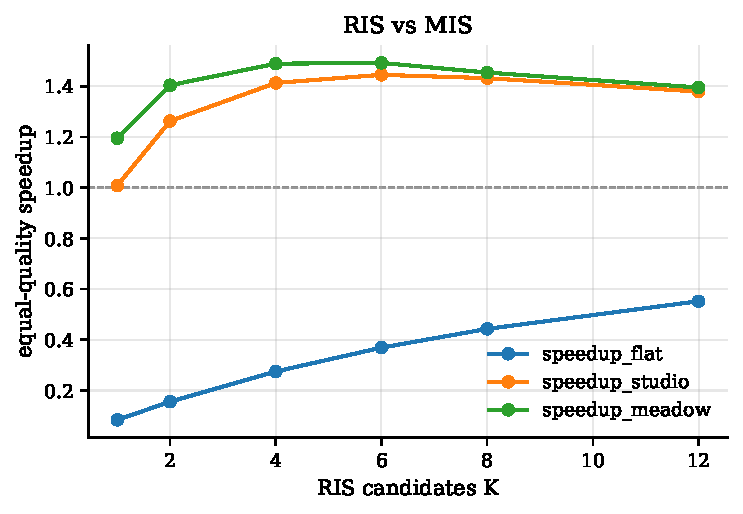
\includegraphics[width=0.8\linewidth]{figures/ris_ksweep.pdf}
  \caption{Volumetric product-RIS versus plain MIS at equal quality, as the candidate count $K$
varies, across three environments of increasing peakiness: flat (constant), studio
(${\sim}540\times$ peak-to-mean), showcase (${\sim}1.5{\times}10^{5}$). The win rises with
peakiness and plateaus at $K=4$--$6$; on flat it is a net loss at every $K$ (the dashed
line marks break-even). Protocol as \Cref{fig:ris-noise}: $k$ from \num{16} seeds at
\num{64}\,spp per $K$, frame times from interleaved rounds, speedup $=$ the $k\cdot t$
ratio. Hence the runtime flag (default plain MIS).}
  \label{fig:ris-ksweep}
\end{figure}

The per-sample variance reduction behind this speedup is visible directly (\Cref{fig:ris-noise}). At
an equal \num{64}-sample budget on the showcase, product-RIS reaches a lower RMSE against the
converged reference image than
plain MIS \emph{and} costs less per sample. The two effects compound to the equal-quality
$1.48\times$ above (the RMSE ratio squared, times the per-sample time ratio).

\begin{figure}[tbp]
  \centering
  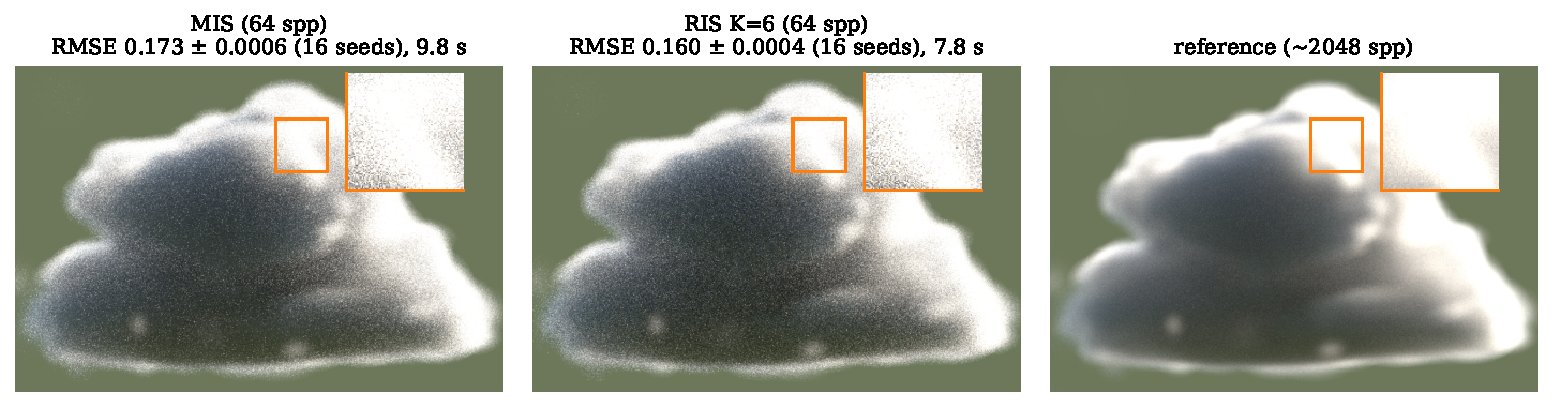
\includegraphics[width=\linewidth]{figures/ris_noise.pdf}
  \caption{Volumetric product-RIS ($K=6$) versus plain MIS on the environment-lit showcase at an equal
  \num{64}-sample budget, against a ${\sim}\num{2048}$-sample reference (the pooled mean of the two
  arms' \num{32} frames; both estimators are unbiased
  here and converge to it). RIS lowers the per-sample RMSE ($\num{0.160}\pm\num{0.0004}$ vs.\
$\num{0.173}\pm\num{0.0006}$; mean $\pm$ standard deviation over \num{16} independent
seeds, the displayed panel being each arm's median seed) and renders faster per sample.
Both wins at once are possible because the baseline pays two shadow rays per vertex where
RIS pays $K$ ray-free evaluations plus one ray. Inset crops show the firefly suppression. The combined equal-quality gain is the $1.48\times$ of \Cref{fig:ris-ksweep}.}
  \label{fig:ris-noise}
\end{figure}

\section{Complexity-argued improvements}
\label{sec:complexity}

The architecture's argmin scatter sampler (\Cref{sec:adt}) improves on the reference asymptotically
rather than by a tuned constant, so it is argued by complexity rather than ablated. There is no on/off
switch to flip: the reference's segment-by-segment marcher is a different algorithm. An ablation
would only confirm what the bound already states: $H$ re-traversals, an ordered $O(H^2)$ boundary
march, and a per-segment
root-find cost more than a single unordered argmin over closed-form free flights (\Cref{tab:complexity}).
One measured anchor grounds the traversal term. The cap-free experiment (\Cref{sec:autopsies}) added
a \emph{single} bounded re-traversal per bounce, and that alone cost $+12$--$22\,\%$ frame time on
the smaller assets.
The supporting $O(1)$ bit-vector active set is justified the same way (\Cref{sec:gpu-impl}); the
active-set inheritance that removes the residual per-bounce $O(N)$ containment scan is, by contrast, a
measured win (\Cref{tab:wins}).

\begin{table}[htp]
  \centering
  \begin{tabular}{@{}lll@{}}
    \toprule
    Per-bounce step & Reference (marching) & This renderer (argmin) \\
    \midrule
    Traversals          & $H$ (one per entry)      & $1$ (single any-hit) \\
    Boundary selection  & $O(H^2)$ boundary re-scan & eliminated (unordered) \\
    Scatter distance    & bisection in overlaps    & closed-form $\operatorname{erf}^{-1}$ \\
    \bottomrule
  \end{tabular}
  \caption{One bounce of a ray crossing $H$ primitives: the reference's segment marcher versus the
argmin sampler (\Cref{fig:pipeline}). Each row is justified by its bound rather than an
ablation: one any-hit traversal replaces $H$ re-traversals; the ordered $O(H^2)$ boundary
re-scan becomes one unordered $O(H)$ reduction; and the scatter distance inverts in closed
form even across overlaps, where the reference falls back to bisection. The active-set
inheritance that removes the residual per-bounce $O(N)$ scan is a \emph{measured} win
(\Cref{tab:wins}).}
  \label{tab:complexity}
\end{table}

\section{Decisions justified without ablation}
\label{sec:reasoned}

Some choices are deliberately \emph{not} measured. Standard-practice optimisations are cited rather
than ablated: multiple CUDA
streams with asynchronous transfers, fused multiply-adds and loop unrolling, \texttt{float4}-coalesced
buffers, the fast-math flag set, GAS compaction and
\texttt{PREFER\_FAST\_TRACE}~\cite{CudaBestPractices,Optix}. Measuring them
would re-derive textbook results---for example, regressing to a single CUDA stream. One
design decision, by contrast, deserves a direct measurement rather than an argument: analytic versus
tessellated sphere geometry. Porting the historical icosphere mesh into the current renderer behind a
build switch yields an A/B in which only the per-primitive geometry differs (\Cref{sec:icosphere}).

\section{Analytic versus tessellated primitive geometry}
\label{sec:icosphere}

\textbf{Goal:} settle the per-primitive geometry choice (the reference's tessellated shell or the
analytic sphere) by a controlled head-to-head.
The reference~\cite{DSYG} renders each primitive as a \emph{tessellated icosphere}, reporting up to a $4.96\times$ speedup over its own custom ray-ellipsoid intersector; its
shell ablation (its Fig.~12) tests icospheres up to \num{320} triangles and finds the
\num{320}-triangle icosphere the best trade-off. This renderer instead uses OptiX's built-in \emph{analytic} sphere
over a single instanced unit GAS. It also supports the tessellated icosphere behind a compile switch,
so the two geometries can be measured head-to-head with the per-primitive geometry the \emph{only}
difference.

\textbf{Setup:} the A/B ports the icosphere mesh (subdivision level $\ell$: \num{20}, \num{80}, \num{320},
\num{1280} triangles). The IAS instancing, the any-hit entry collection,
and the analytic optical-depth integration are untouched, with one addition. A convex shell is
entered through a front face and left through a back face; the any-hit therefore keeps only
front-face hits, preserving the one-entry-per-primitive contract the sphere provides natively.

\begin{table}[htp]
  \centering
  \setlength{\tabcolsep}{4pt}%
  \begin{tabular}{@{}lrrrrrr@{}}
    \toprule
    & & \multicolumn{2}{c}{frame time (cloud)} & \multicolumn{3}{c}{RMSE vs analytic} \\
    \cmidrule(lr){3-4} \cmidrule(l){5-7}
    Shell & tris & abs. & rel. & cloud & tornado & bunny \\
    \midrule
    \textbf{analytic sphere} & --- & \textbf{\SI{15.52}{\second}} & \textbf{$1.00\times$} & \textbf{0} & \textbf{0} & \textbf{0} \\
    icosphere $\ell{=}0$ & 20   & \SI{9.80}{\second}  & $0.63\times$ & $4.0\times10^{-2}$ & $9.5\times10^{-3}$ & $1.2\times10^{-2}$ \\
    icosphere $\ell{=}1$ & 80   & \SI{11.22}{\second} & $0.72\times$ & $1.0\times10^{-2}$ & $2.0\times10^{-3}$ & $2.7\times10^{-3}$ \\
    icosphere $\ell{=}2$ & 320  & \SI{11.99}{\second} & $0.77\times$ & $2.5\times10^{-3}$ & $4.7\times10^{-4}$ & $6.3\times10^{-4}$ \\
    icosphere $\ell{=}3$ & 1280 & \SI{13.23}{\second} & $0.85\times$ & $8.2\times10^{-3}$ & $5.2\times10^{-3}$ & $4.3\times10^{-3}$ \\
    icosphere $\ell{=}4$ & 5120 & ---                 & ---          & $9.6\times10^{-3}$ & $5.5\times10^{-3}$ & $4.8\times10^{-3}$ \\
    \bottomrule
  \end{tabular}
  \caption{Analytic built-in sphere versus tessellated icosphere, with only the per-primitive geometry
  differing. The shipped configuration (\textbf{analytic sphere}, bold) is kept for its exactness, at
$1.17$--$1.58\times$ the frame time of every tessellated level. Frame times: cloud
  scattering under the environment-lit showcase, \num{128} spp, median of five interleaved rounds at
  locked clocks (within-arm spread ${\le}1.5\,\%$); $\ell{=}4$ was measured for accuracy only and carries no timed row. RMSE: absorption renders against the
  analytic render, which is exact here---the instanced primitive \emph{is} a sphere---so the residual is
  pure tessellation error. Absorption renders are deterministic (\Cref{sec:setup}), so these numbers
  carry no seed variance.}
  \label{tab:icosphere}
\end{table}

\textbf{Result---throughput.} Which geometry is cheaper here was not obvious in advance. The analytic
sphere is the single instanced unit-sphere GAS of \Cref{sec:gpu-impl}---one primitive,
transformed per instance, against a mesh duplicated per primitive---and is intersected by
OptiX's built-in sphere routine. On the timing question, \Cref{tab:icosphere} favours the
tessellated shell: it is \emph{faster at every tessellation level}, and the analytic sphere pays $1.17$--$1.58\times$ in frame time for its exactness. The
mechanism is the one the DSYG paper itself identified~\cite{DSYG}. On RTX-class hardware,
ray-triangle intersection runs on the
dedicated ray-tracing cores; the built-in sphere is intersected by a \emph{software} routine on
the otherwise hardware-accelerated traversal path. The A/B was still necessary: the paper's
$4.96\times$ is measured against a different analytic baseline, so the magnitude---and with it
the decision---had to be established here. Indeed it comes out far smaller. Their analytic arm
was a custom \emph{software} ellipsoid intersector over per-primitive world-space bounds;
anisotropic primitives inflate those axis-aligned boxes, so traversal tests many primitives a
ray misses. This renderer's analytic arm starts from a much stronger position: the instanced
unit-sphere GAS with tight per-instance transforms.

\textbf{Result---accuracy.} Accuracy behaves oppositely, and non-monotonically. From $\ell{=}0$ to $\ell{=}2$ the error falls
${\sim}4\times$ per subdivision with the physically expected sign. The tessellation's vertices lie on
the sphere and its faces are chords inside it. The shell is therefore slightly smaller than the true
$3\sigma$ ellipsoid, and the renders are marginally too bright. At $\ell{=}3$ the
error \emph{rises} on all three assets and flips sign to \emph{darker}
(\Cref{fig:icosphere-sliver}). The mechanism is geometric. Near a primitive's silhouette the
shell's triangles are seen edge-on, and each subdivision makes them longer and thinner---slivers. A
ray that grazes the shell meets such a sliver at near-parallel incidence. At that incidence the
intersection arithmetic is ill-conditioned along the sliver's long axis: in single precision,
rounding can slide the computed entry point far \emph{along} the triangle. The renderer is then
told the ray entered the primitive somewhere it did not.
Every downstream quantity (the analytic exit, the chord, the optical depth) is computed from that
entry, so one bad entry mis-integrates that ray's whole contribution. (The mechanism is inferred from the image evidence---the errors sit at silhouettes, flip sign, and grow with
subdivision; the intersection arithmetic itself was not instrumented.) Only grazing rays
are affected, so the error is a thin band of wrong pixels along each silhouette rather than
an image-wide bias. The affected-pixel count accordingly tracks per-primitive
screen footprint rather than anisotropy---the round-primitive cloud, whose large Gaussians have the
most silhouette pixels per primitive, is hit hardest. Because these are deterministic absorption renders, the effect is
exactly reproducible. An added $\ell{=}4$ level continues the trend: both the error and the
affected-pixel population keep growing (\Cref{fig:icosphere-sliver}). Past $\ell{\approx}2$,
finer tessellation is both slower and less accurate---consistent with the reference's
shell ablation never going beyond \num{320} triangles.

The decision, then, is a genuine accuracy-versus-performance trade, and this renderer keeps the
analytic sphere for correctness, at the $1.17$--$1.58\times$ frame-time cost measured above. Even the best shell
($\ell{=}2$) brightens the whole cloud image by ${\sim}0.16\,\%$---invisible to the eye.
But that is an order of magnitude above the $10^{-4}$-level energy agreement that the validation gates of
\Cref{ch:validation} hold the renderer to. The analytic shell makes those gates attainable.
Where raw throughput matters more than validation-grade exactness,
$\ell{=}2$---the reference's own \num{320}-triangle choice---is the right shell.
The instanced single-GAS design keeps even that choice memory-trivial: \SI{9.6}{\kilo\byte} compacted,
versus per-primitive duplication in the reference.

\begin{figure}[t]
  \centering
  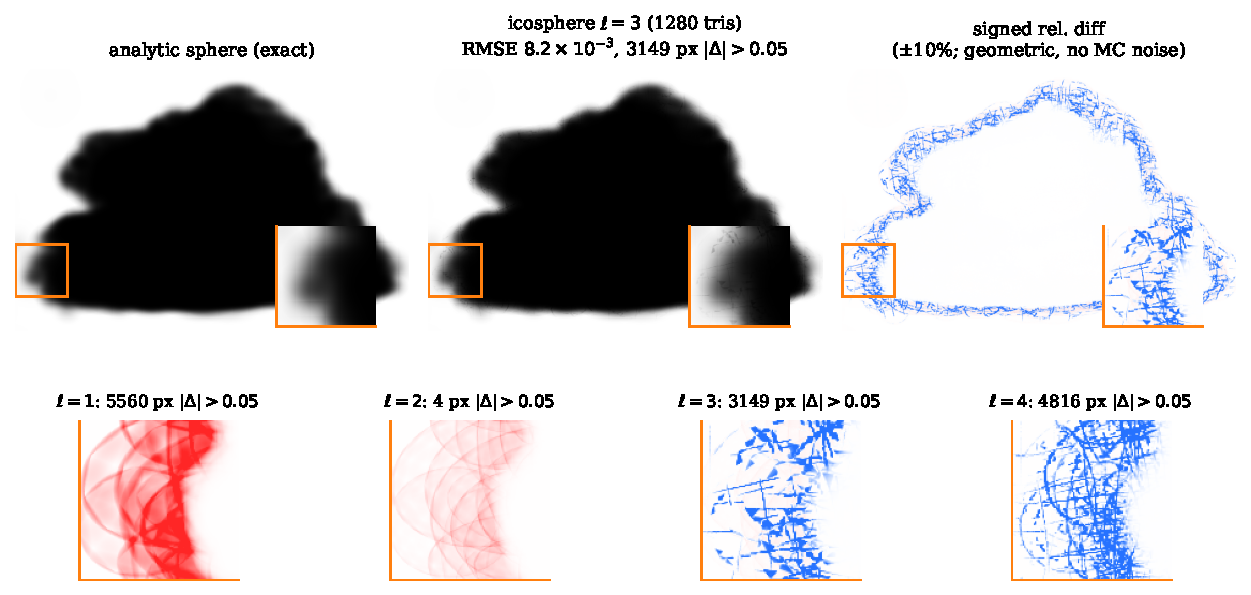
\includegraphics[width=\linewidth]{figures/icosphere_sliver.pdf}
  \caption{The $\ell{=}3$ sliver artefact (cloud, pure absorption, so transmittance is deterministic and
  every difference is geometric, not Monte Carlo noise). \emph{Top, left to right:} the analytic
  sphere (exact); the \num{1280}-triangle icosphere, whose inset crop shows faceted slivers where the
  analytic shell is smooth; and the signed relative difference ($\pm\num{10}\,\%$ full scale; conventions,
\Cref{sec:setup})---the error is a thin band of silhouette pixels (\num{3149} at
$|\Delta|>0.05$, peak $|\Delta|\approx0.25$). \emph{Bottom:} the same crop's signed difference across
  $\ell=1\ldots4$, showing the two error regimes: the smooth \emph{faceting} bias (red: tessellated
  shell brighter) shrinks with subdivision and nearly vanishes at $\ell{=}2$ (\num{4} pixels above
  threshold), then the \emph{sliver} population (blue: darker, jagged) appears at $\ell{=}3$ and
  grows at $\ell{=}4$ (\num{3149}$\to$\num{4816} pixels). All panels are from the runs behind \Cref{tab:icosphere}.}
  \label{fig:icosphere-sliver}
\end{figure}

\section{Negative results}
\label{sec:autopsies}

The following ideas were implemented or seriously evaluated and did not pay off. Each is reported as
hypothesis, cheap kill-test, measurement, and lesson.

\begin{itemize}
  \item \textbf{Wavefront refactor --- the largest regression.} Splitting the megakernel into per-stage
  kernels makes the renderer ${\sim}100\times$ \emph{slower}: an interleaved A/B on the
  scattering cloud (\num{4}\,spp, binaries rebuilt from the archived branch) measures the
  wavefront build at over a hundred times the megakernel's frame time. The roughly \num{352} bytes of per-ray state (hit buffer, active set, and live
locals---the exact total shifts with compiler allocation) must stream through DRAM
  every bounce, and it goes super-linear once the working set exceeds L2. \emph{Lesson:} moving persistent
  per-ray state to global memory is fatal for this workload: the state belongs in registers,
inside one kernel, and this rules out the family of designs that would stream it
(wavefront, ray-sorting, neural caches).
  \item \textbf{Megakernel footprint reduction.} Structure-of-arrays (SoA) layouts, field
  reordering, and read-only-cache load hints (\texttt{\_\_ldg}) were null: the data is already
  cache-resident, so the cost is load
  \emph{latency}, not footprint. The same diagnosis closed \emph{half-precision compression} of the
  primitive fields before implementation. An fp16 round-trip of the optical-thickness, albedo,
  and normalisation fields is accuracy-safe ($\le 3.3\times10^{-4}$ relative).
  But the whole primitive array is ${\le}\num{0.25}\,\%$ of device memory (\SI{52}{\kilo\byte} on
  the cloud, \SI{2.0}{\mega\byte} on the bunny) and, per the above, already cache-resident.
  Halving it moves nothing that matters, and the hot \num{64}-byte struct layout was left
  undisturbed.
  \item \textbf{Cap-free streaming scatter sampling.} The hit
  buffer is written once and read twice (\Cref{sec:adt}): once for the argmin, once to rebuild the
  active set at the scatter point. The first read never needed a buffer: a minimum is an
  order-independent reduction, computable on the fly. In principle the buffer can therefore be
  deleted. The rewrite streams the argmin inside the any-hit shader, computing each primitive's
  free-flight draw the moment traversal reports it. It replaces the second read with one more
  \emph{bounded} re-traversal, capped at the sampled scatter distance $t^\star$, that re-tests
  which primitives span the scatter
  point. Per-ray
  sampling state falls to $O(1)$ and there is no hit-buffer capacity to tune. One subtlety makes the rewrite testable at all. It was held to the strongest regression
standard: reproduce the buffered sampler's images bit for bit, not merely statistically.
Each primitive's free-flight proposal consumes one uniform $\xi_k$ (\Cref{sec:adt}), and a
sequential generator hands the uniforms out in processing order---an order the two
implementations do not share, since traversal reports hits in no guaranteed order. The hit
set and the argmin are order-independent, so both samplers are correct; but which $\xi$
lands on which primitive differs, so the two images differ in their noise and can never be
compared bit for bit. Each $\xi_k$ is therefore computed as a stateless hash of its
consumer's identity---path, bounce, primitive---in the spirit of counter-based
generators~\cite{Salmon2011}. Every primitive then receives the same uniform in both
implementations, in any processing order, and any remaining image difference is a real
defect. The
  reformulation was indeed validated to \emph{bit-exactness} against the buffered sampler (furnace plus all
  four assets). It rendered the entire lineup with one stock binary and zero overflows. And it still lost
  the interleaved A/B against the per-asset-tuned baseline: $+22\,\%$ frame time on the tornado,
  $+16\,\%$ explosion, $+12\,\%$ cloud, $-2\,\%$ bunny. The profile explains why: local-memory
  traffic fell ($-8\,\%$ L2 bytes) but instructions rose ($+6\,\%$) at \emph{unchanged} occupancy.
  The kernel is register-limited, so local-memory savings cannot buy parallelism. The extra
  bounded re-traversal plus per-hit any-hit transitions are pure added work on small assets.
  \emph{Lesson:} a cleaner memory shape gains nothing while occupancy is bounded by
registers rather than local memory. Although the variant was abandoned, its bit-exactness
validation exposed two latent bugs in this renderer's own production path. The experiment advanced through a
  sequence of increasingly strict gates, each requiring bit-exact agreement with the buffered sampler.
  That gate exposed a silent-bias bug in the \emph{original, buffered} path. For random draws near zero, rounding could land the sampled scatter distance just before
the winning primitive's own entry point---a position it can mathematically never precede. The winner was then
  wrongly dropped from its own scatter's candidate set, silently killing the path (since fixed).
  The same gate established empirically that OptiX does not report hits at exactly
  $t = t_{\max}$---an endpoint behaviour the OptiX documentation does not specify.
  \item \textbf{Adaptive sampling.} Per-pixel convergence stopping was a net loss. At the
  working threshold nothing early-stops on the high-variance cloud. It therefore matches uniform
  sampling at identical quality but runs \num{0.9}\,\% slower (\num{0.7}\,\% on the calibrated-caps
  re-confirmation) and reserves an extra per-pixel variance buffer. A
  more aggressive threshold only trades that overhead for firefly bias. Kept, default-off.
  \item \textbf{Per-step Rao--Blackwellisation.} The renderer
  is \num{1.6}$\times$ noisier per sample than Mitsuba at matched reconstruction filters on the
  flat-lit scattering cloud (\Cref{sec:results-perf}).\footnote{The investigation predated the filter matching of \Cref{sec:results-perf} and was
motivated by a since-withdrawn ${\sim}5\times$ unmatched-filter reading (footnote 3
there).} The hypothesis attributed the gap to Mitsuba folding the analytic segment transmittance
  into throughput at \emph{every} bounce, versus only at the primary vertex here. Varying a single Gaussian's optical depth, and measuring both estimators' per-sample
variance at each point, isolated the effect from overlap and from environment sampling; as
a control, disabling MIS
  moved the noise by only $1.06\times$. The sweep confirmed a real gap but corrected its cause.
  The reference lets every path carry a
  fractional ``how much light survives'' weight to its end, while the argmin flips a hard
  scatter-or-escape coin at each step (\Cref{sec:adt}). An average of smooth fractions is
  quieter than an average of coin flips. Both are classical transmittance estimators of transport Monte Carlo. Binary scores are the
higher-variance family, and replacing the termination coin flip by its continuation
weight---known as \emph{implicit capture} or \emph{Rao--Blackwellisation}---is the
classical remedy~\cite{Novak2018}; the gap \emph{widens with depth}. Under flat lighting at
the test's albedo \num{0.9} (little absorption), nearly every reference sample already
lands near the mean---its smooth weight varies little---while the coin flip keeps its full
spread.
  The fix is declined on two grounds. First, the obvious patch
  (adding the continuation escape as a second sampling strategy) replaces the existing \emph{analytic}
  shadow-ray next-event estimator with a higher-variance \emph{stochastic} escape indicator (same
  expectation, strictly worse). Second, folding transmittance into throughput at every bounce would abandon
  the binary scatter/escape decision at the core of the sort-free argmin. \emph{Lesson:} a characterised
  trade-off, not a missed optimisation. It helps only the flat-lighting regime (a uniform
  environment), while the environment-lit
  showcase (the target) is already won by MIS (\Cref{ch:results}). One hybrid remains untested:
  keep the argmin's single trace for choosing scatter points, but also carry the analytic
  segment transmittance in the path weight at every bounce, reweighted to stay unbiased. It was not built here: the flat-lighting regime it would help
is not the target regime, and the showcase comparison is already in this renderer's favour
without it. Whether it inherits
the smooth-weight benefit without a new cost is therefore unknown; it is the direction to
try should the flat gap ever matter.
  \item \textbf{Density-contribution culling.} Hypothesis: skip primitives whose density
  contribution along the chord is negligible before integrating them. Null: the BVH reports only
  primitives whose $3\sigma$ support the ray actually enters, so the cull re-tests what traversal
  already guarantees.
  \item \textbf{Weighted-escape combine.} Hypothesis: estimate the environment term
  twice---once by the existing analytic shadow-ray term, once by a reference-style stochastic
  escape weight---and combine the two estimators. Null: the analytic term already has zero
  variance, so a stochastic partner can only add noise.
  \item \textbf{Exit-caching.} Hypothesis: cache each primitive's exit solution instead of
  recomputing it on demand. Null: bit-identical output and no speedup---the cache's extra per-ray
  state pressed on the same register/occupancy wall as everything else (\Cref{sec:bottleneck}).
  \item \textbf{Env-IS alias table.} Hypothesis: $O(1)$ alias-method sampling of the environment map, replacing the binary
search through the map's cumulative-distribution table. Null: correct but sub-$1\%$---environment sampling is
  nowhere near the bottleneck.
  \item \textbf{Owen--Sobol sampling.} Hypothesis: low-discrepancy (Owen-scrambled Sobol) sequences
  in place of pseudo-random numbers. Null: no measurable win. The variance is dominated by rare high-energy scattering events,
which better-spread samples do not hit more often; and a volumetric path consumes many
random dimensions, where low-discrepancy points lose their edge.
  \item \textbf{Path guiding.} Path guiding learns, during rendering,
  where light actually arrives from. The radiance carried by completed paths is recorded into a
  spatial-directional structure (in practical form, an adaptive SD-tree over the
  scene~\cite{Muller2017}). Scatter directions are then drawn from that learned distribution
  instead of the phase function alone. That is valuable when important light arrives, after several
  bounces, from directions the phase function does not favour. Here the case was weak on three
  fronts. First, no \emph{cheap} trial could validly predict its gain: cheap proxies only probe the direct light that NEE already handles, while guiding's payoff lies in light arriving
after several bounces. Second, the upside is bounded low: after a few scatters the deep interior is near-diffuse
(light arrives roughly equally from all directions), so there is little directional
structure to learn, while MIS already handles the dominant sun. Third, the learned structure must live in global memory and be
  queried at every bounce---exactly the per-ray-state externalisation \Cref{sec:bottleneck}
  punishes. Building it would have been a multi-day bet against weak evidence. Unlike the
  entries above, this is therefore a judgment call, not a measurement: the idea is deferred,
  and it remains the best-motivated next step should strongly directional deep transport ever matter.
\end{itemize}

The unifying lesson is the bottleneck of \Cref{sec:bottleneck}: at low occupancy bound by global-load
latency, footprint and cache micro-optimisations are near-null, and any restructuring that externalises
per-ray state backfires. The best-suited hardware lever for this divergence---OptiX Shader Execution
Reordering~\cite{NvidiaSER2022}---is Ada-only and therefore unavailable on the Ampere RTX~3090 used here.
\Cref{sec:ser} measures on an Ada GPU what it recovers.

\section{Shader Execution Reordering: a cross-architecture probe}
\label{sec:ser}

\textbf{Goal:} quantify, on hardware that has it, what SER recovers of the divergence cost
diagnosed in \Cref{sec:bottleneck}.
The reordering mechanism named above---OptiX Shader Execution Reordering (SER)---is a hardware
feature of the Ada generation (compute capability~8.9) and later, unavailable on the Ampere
RTX~3090 this thesis is pinned to. Its effect is therefore measured on Ada directly. At a
programmer-inserted point, SER repartitions the in-flight threads of a launch into fresh warps grouped by a
\emph{coherence key}, then resumes them. A warp left incoherent by a divergent trace becomes coherent for the
shading and next-bounce work that follows. That restores lane utilisation and coalesces the scattered
\texttt{Primitive} loads that \Cref{sec:bottleneck} identified as the bottleneck. Two properties make it a clean test of that diagnosis. It is \emph{pure scheduling}: it
changes which threads co-execute, not what each computes, so the image is bit-identical.
And the reference cannot apply it. Mitsuba
renders through Dr.Jit, which compiles one fused megakernel from a high-level trace and emits no reorder
points. This renderer's hand-written argmin megakernel can place a single \texttt{optixReorder}
after the scatter event, precisely because it controls its own trace structure.

\textbf{Setup:} the renderer was built with SER enabled: one reorder per bounce.\footnote{A
compile-time switch---the production binaries used everywhere
else in this thesis contain no reorder call.} The reorder's default grouping is by hit; this
build supplies its own coherence key, a hash of the quantised scatter position, so rays that
scattered near one another regroup. It ran against the identical SER-off build on a rented
RTX~4090, at each asset's
calibrated caps. The rented host permits neither profiling counters nor clock pinning, so, unlike
every \num{3090} figure, the 4090's operating point could not be locked. The comparison is
wall-clock, with the interleaving as the drift control: warm-up
plus eleven interleaved off/on repetitions at \num{64}\,spp, reporting the median. As expected,
every SER-on image was verified bit-identical to its SER-off counterpart, so the wall-clock
ratio is also the equal-quality ratio.

\begin{table}[htp]
  \centering
  \begin{tabular}{@{}lrrr@{}}
    \toprule
    Asset & SER-off (s) & SER-on (s) & Speedup \\
    \midrule
    cloud     & 3.274  & 2.303  & $1.42\times$ \\
    explosion & 2.644  & 1.877  & $1.41\times$ \\
    tornado   & 3.060  & 2.729  & $1.12\times$ \\
    bunny     & 22.674 & 13.494 & $\mathbf{1.68\times}$ \\
    \bottomrule
  \end{tabular}
  \caption{Shader Execution Reordering on an RTX~4090, per asset at calibrated caps, \num{64}\,spp,
median of eleven interleaved wall-clock repetitions (quoted to the millisecond so each
speedup reproduces from its row; per-repetition times were not retained). Every SER-on image is bit-identical to SER-off, so each speedup is also an equal-quality
speedup; largest speedup in bold. Cloud hint ablation: the scatter-cell key (a \num{256}-bucket hint from the position on a
$\tfrac{1}{8}$-unit grid) gives $1.42\times$, the hintless \texttt{optixReorder()}
$1.25\times$, reordering at the first bounce only $1.10\times$; under product-RIS the
cloud win is $1.35\times$.}
  \label{tab:ser}
\end{table}

\textbf{Result:} SER helps on every asset: \num{1.12} to \num{1.68}$\times$ (\Cref{tab:ser}). The
magnitude tracks the amount of divergent \emph{shading} work rather than how sparse the asset is. It is largest on
the dense, deeply-overlapped bunny ($1.68\times$) and smallest on the thin, mostly-empty tornado
($1.12\times$), whose rays escape quickly and leave little shading to regroup. Even the hintless \texttt{optixReorder()} helps: $1.25\times$ on the cloud, grouping by
hit alone. The scatter-cell key raises that to $1.42\times$. Reordering at \emph{every} bounce, not just the first, is likewise what carries the gain
($1.10\times$ for bounce-0 alone). The win persists under the production direct-lighting estimator
($1.35\times$ with product-RIS). The result confirms the \Cref{sec:bottleneck} diagnosis
directly: the one mechanism designed for this exact failure mode---warp divergence on
scattered loads---removes \num{11}--\num{40}\,\% of the frame time (the
\num{1.12}--\num{1.68}$\times$ are throughput factors). It also exposes an
\emph{architectural} advantage: on SER-capable hardware this renderer pulls further ahead,
because its hand-authored kernel can request reordering and the reference's generated
pipeline cannot.

\paragraph{From a mechanism to an end-to-end advantage.}
The architectural gap that SER widens can be stated end-to-end on the Ada host. The renderer's noise
constant reproduced the \num{3090} value to the three decimals recorded
($k_{\text{clip}}=\num{1.887}$ on both hosts), as it must: $k$ depends only on the
sampler and the scene. Only per-sample time therefore changes across
architectures, and every figure below is traceable. On that host this renderer takes the \num{64}-spp showcase of \Cref{fig:showcase} from
\SI{3.29}{\second} to \SI{1.63}{\second} end-to-end ($2.0\times$); \Cref{tab:ser-eq} lists
the steps.
Because SER is
image-identical and the other steps sit inside the validation gates, each render-time step is also an
equal-quality step. The like-for-like headline of \Cref{sec:results-perf} remains the \num{3090}
figure, which these Ada measurements extend and do not alter.

\begin{table}[htp]
  \centering
  \resizebox{\linewidth}{!}{%
  \begin{tabular}{@{}lrr@{}}
    \toprule
    configuration & render (s) & step \\
    \midrule
    MIS, no SER                  & 3.29 & --- \\
    MIS $+$ SER                  & 2.31 & $\mathbf{1.42\times}$, image-identical \\
    RIS $+$ fast \texttt{erf} $+$ SER & 1.92 & $1.20\times$, within gates \\
    \quad$+$ icosphere $\ell{=}2$ & 1.63 & $1.18\times$, ${\sim}0.1\%$ systematic \\
    \bottomrule
  \end{tabular}%
  }
  \caption{End-to-end render time of the \num{64}-spp showcase on the Ada host, per configuration
step (median steady-state). SER is image-identical, so its step is an equal-quality
speedup by construction; the RIS/fast-\texttt{erf} and icosphere steps sit inside the
validation gates of \Cref{ch:validation} (the icosphere trades a ${\sim}\num{0.1}\%$
systematic). The rows are the recorded configurations of the probe, not a full ablation
(the combined step is dominated by RIS). The cloud pair (unrounded
\num{3.285}/\num{2.309}) is a separate \num{16}-seed session from \Cref{tab:ser}'s A/B
(\num{3.274}/\num{2.303}); the sessions agree within \num{0.4}\,\%. The like-for-like
headline (\Cref{tab:likeforlike}) lives on the \num{3090} host and is not modified by
these figures.}
  \label{tab:ser-eq}
\end{table}

\section{Memory}
\label{sec:opt-memory}

On the memory side, the acceleration structure is not where the budget goes: it is
sub-megabyte for the cloud and a few megabytes for the bunny, dwarfed by the megakernel's
per-ray state---the same state whose externalisation sank the wavefront attempt
(\Cref{sec:autopsies}). It is built
with compaction as a matter of course (a single
build flag, \texttt{OPTIX\_BUILD\_FLAG\_ALLOW\_COMPACTION}, also used by the reference).

\paragraph{Per-asset capacity budgets.} The per-ray buffers are bounded by the worst-case primitive
overlap a scene presents, which the offline estimator of \Cref{sec:gpu-impl} predicts from geometry
alone. \Cref{tab:overlap} reports that estimate across assets. The overlap varies by more than
$25\times$ and does not track the primitive count. A \num{4096}-primitive cloud fit
demands an order of magnitude more \emph{active-set} capacity (point overlap \num{529} vs \num{57}) than
a \num{24576}-primitive one. Overlap is set by
how densely the Gaussians pack rather than by how many there are. No single static cap fits every scene,
so the caps are per-asset. The primary cloud's calibrated \num{64}/\num{96} buffers would
overflow on the denser fits and the bunny, which therefore compile with their own larger caps,
sized by the estimator ahead of the build (\Cref{tab:vram}).

\begin{table}[htp]
  \centering
  \begin{tabular}{@{}lrrr@{}}
    \toprule
    Asset & Primitives & Max point overlap & Max ray entries \\
    \midrule
    Disney cloud, primary fit & \num{652}   & \num{45}  & \num{96}  \\
    Disney cloud, coarse fit  & \num{768}   & \num{19}  & \num{108} \\
    Disney cloud, dense fit   & \num{4096}  & \num{529} & \num{706} \\
    Disney cloud, fine fit    & \num{24576} & \num{57}  & \num{437} \\
    Tornado                & \num{768}   & \num{84}  & \num{340} \\
    Explosion              & \num{1024}  & \num{23}  & \num{136} \\
    Stanford bunny         & \num{25600} & \num{245} & \num{387} \\
    \bottomrule
  \end{tabular}
  \caption{Worst-case $3\sigma$ overlap per asset, \emph{estimated} offline by the cap estimator. These
  geometric predictions seed the compile-time caps (\texttt{MAX\_ACTIVE\_PRIMS} from point overlap,
  \texttt{HIT\_BUFFER\_CAPACITY} from ray entries), but they are estimates and carry no guarantee: where the
  in-render counters disagree, the counters are the sizing authority (\Cref{sec:gpu-impl}). The bunny is the clear case: the estimator over-predicts its point overlap (\num{245}
vs.\ \num{71} measured, shipped at \num{80}) and under-predicts its ray entries (\num{387}
vs.\ \num{464} measured, shipped at \num{528}). Shipped caps (\Cref{tab:vram}) are sized
from the measured maxima by a $\times1.125$ pad rounded up to the next multiple of
\num{16}, then verified overflow-free on an unmeasured seed. The four cloud rows are
distinct density fits of the same volume.}
  \label{tab:overlap}
\end{table}
